\section{\textit{Kernel}, qual a importância?} \label{section: kernel}

\subsection{O que é?}
O \textit{Kernel} é um componente fundamental de qualquer sistema operacional, sendo responsável pela gestão dos recursos de hardware e por fornecer uma interface entre o software e o hardware do computador. \cite{kernel}

\begin{figure}[H]
  \centering
  % width=\textwidth para imagem da largura do texto
  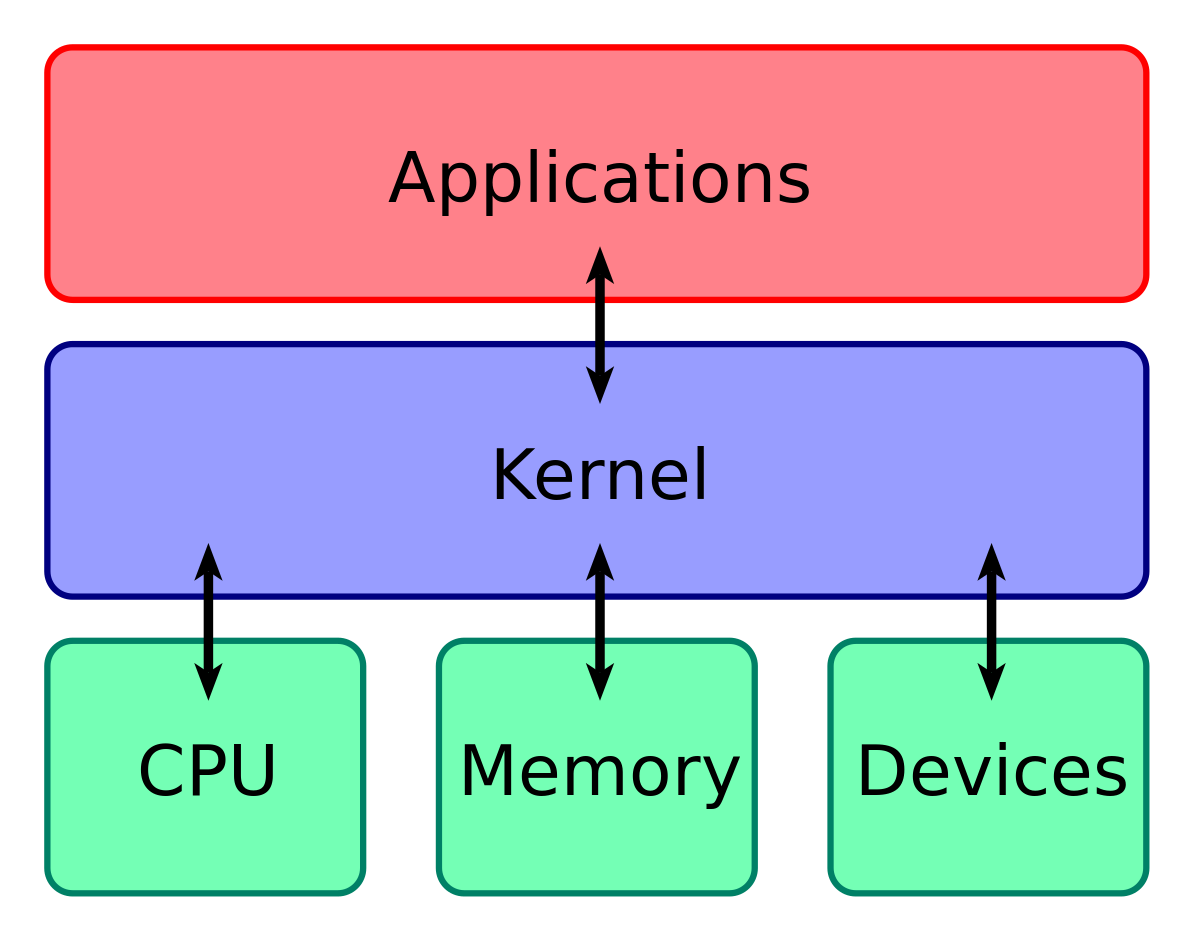
\includegraphics[scale=0.2]{Figures/0. General/kernel.png}
  \caption{Simplificação de como opera o \textit{Kernel}}
  \label{Simplificação da operação do Kernel}
\end{figure}

\subsection{Importância}
Algumas das responsabilidades do \textit{Kernel} são:

\begin{itemize}

  \item \textbf{Gestão de recursos}\\
  O \textit{Kernel} é responsável pela alocação e gestão dos recursos de hardware, garantindo que os processos em execução no sistema tenham acesso adequado à CPU, memória e dispositivos periféricos.

  \item \textbf{Abstração de hardware}\\
  O \textit{Kernel} fornece uma camada de abstração entre o software e o hardware, permitindo que os desenvolvedores de aplicativos escrevam código independente de plataforma. Isso facilita o desenvolvimento de software portátil e compatível com diferentes sistemas operativos.

  \item \textbf{Execução de tarefas do sistema}\\
  O \textit{Kernel} é responsável pela execução de tarefas essenciais do sistema, como o agendamento de processos, gestão de memória virtual, gestão de interrupções e controlo de dispositivos de entrada e saída.

  \item \textbf{Segurança e proteção}\\
  O \textit{Kernel} implementa mecanismos de segurança e proteção para garantir a integridade e a segurança do sistema e dos dados dos utilizadores. Controla o acesso aos recursos do sistema e impede que processos maliciosos comprometam a estabilidade do sistema.

  \item \textbf{Desempenho e eficiência}\\
  Um \textit{Kernel} eficiente é essencial para o desempenho e a eficiência do sistema operativo como um todo. Deve ser otimizado para minimizar o tempo de resposta, maximizar a utilização dos recursos de hardware e garantir uma experiência de utilizador fluída.
\end{itemize}
